%  LaTeX support: latex@mdpi.com 
%  For support, please attach all files needed for compiling as well as the log file, and specify your operating system, LaTeX version, and LaTeX editor.

%=================================================================
\documentclass[remotesensing,article,submit,pdftex,moreauthors]{Definitions/mdpi} 

%=================================================================
% MDPI internal commands - do not modify
\firstpage{1} 
\makeatletter 
\setcounter{page}{\@firstpage} 
\makeatother
\pubvolume{1}
\issuenum{1}
\articlenumber{0}
\pubyear{2024}
\copyrightyear{2024}
%\externaleditor{Academic Editor: Firstname Lastname}
\datereceived{ } 
\daterevised{ } % Comment out if no revised date
\dateaccepted{ } 
\datepublished{ } 
%\datecorrected{} % For corrected papers: "Corrected: XXX" date in the original paper.
%\dateretracted{} % For corrected papers: "Retracted: XXX" date in the original paper.
\hreflink{https://doi.org/} % If needed use \linebreak
%\doinum{}
%\pdfoutput=1 % Uncommented for upload to arXiv.org
%\CorrStatement{yes}  % For updates


%=================================================================
% Add packages and commands here. The following packages are loaded in our class file: fontenc, inputenc, calc, indentfirst, fancyhdr, graphicx, epstopdf, lastpage, ifthen, float, amsmath, amssymb, lineno, setspace, enumitem, mathpazo, booktabs, titlesec, etoolbox, tabto, xcolor, colortbl, soul, multirow, microtype, tikz, totcount, changepage, attrib, upgreek, array, tabularx, pbox, ragged2e, tocloft, marginnote, marginfix, enotez, amsthm, natbib, hyperref, cleveref, scrextend, url, geometry, newfloat, caption, draftwatermark, seqsplit
% cleveref: load \crefname definitions after \begin{document}

%=================================================================
% Please use the following mathematics environments: Theorem, Lemma, Corollary, Proposition, Characterization, Property, Problem, Example, ExamplesandDefinitions, Hypothesis, Remark, Definition, Notation, Assumption
%% For proofs, please use the proof environment (the amsthm package is loaded by the MDPI class).

%=================================================================
% Full title of the paper (Capitalized)
\Title{Robot Team III: Scotty Strikes Back}

% MDPI internal command: Title for citation in the left column
\TitleCitation{Title}

% Author Orchid ID: enter ID or remove command
\newcommand{\orcidauthorA}{0000-0002-5910-0183} % John
\newcommand{\orcidauthorB}{0000-0003-2688-648X} % Lakitha
\newcommand{\orcidauthorC}{0000-0002-9841-6703} % Shawhin
\newcommand{\orcidauthorD}{0000-0003-2657-3416} % Prabuddha
\newcommand{\orcidauthorE}{0000-0003-4265-9543} % David
\newcommand{\orcidauthorF}{0000-0003-0667-2345} % Ash
\newcommand{\orcidauthorG}{0000-0002-0126-218X} % Adam
% \newcommand{\orcidauthorH}{} % Gokul

% Authors, for the paper (add full first names)
\Author{John Waczak \orcidA{}, Adam Aker \orcidG{}, Lakitha O. H. Wijeratne \orcidB{}, Shawhin Talebi \orcidC{}, Ashen Fernando \orcidF{}, Prabuddha M. H. Dewage \orcidD{}, Mazhar Iqbal, Matthew Lary, David Schaefer, Gokul Balagopal, and David J. Lary *\orcidE{}}

%\longauthorlist{yes}

% MDPI internal command: Authors, for metadata in PDF
\AuthorNames{John Waczak, Adam Aker, Lakitha O. H. Wijeratne, Shawhin Talebi, Bharana Fernando, Prabuddha Hathurusinghe, Mazhar Iqbal, Matthew Lary, David Schaefer, Gokul Balagopal, and David J. Lary}

% MDPI internal command: Authors, for citation in the left column
 \AuthorCitation{Waczak, J.; Aker, A.; Wijeratne, L.O.H.; Talebi, S.; Fernando, B.; Hathurusinghe, P.; Iqbal, M.; Lary, M.; Schaefer, Balagopal, G.; D.; Lary, D.J.}
% If this is a Chicago style journal: Lastname, Firstname, Firstname Lastname, and Firstname Lastname.

% Affiliations / Addresses (Add [1] after \address if there is only one affiliation.)
\address[1]{%
Hanson Center for Space Sciences, University of Texas at Dallas, Richardson, TX 75080, USA;  john.waczak@utdallas.edu (J.W.); adam.aker@utdallas.edu (A.A.); lhw150030@utdallas.edu (L.O.H.W.); shawhintalebi@gmail.com (S.T.); ashen.fernando@utdallas.edu  (B.F.); pxh180012@utdallas.edu (P.M.H.D.); mazhar.iqbal@utdallas.edu (M.I.); MDL210001@utdallas.edu (M.L.); captdaveschaefer@gmail.com (D.S.); gokul.balagopal@utdallas.edu (G.B.);}

% Contact information of the corresponding author
\corres{Correspondence: david.lary@utdallas.edu} %; Tel.: (optional; include country code; if there are multiple corresponding authors, add author initials) +xx-xxxx-xxx-xxxx (F.L.)}


% Abstract (Do not insert blank lines, i.e. \\) 
\abstract{FIXME}

% Keywords
\keyword{FIXME} 


%%%%%%%%%%%%%%%%%%%%%%%%%%%%%%%%%%%%%%%%%%
\begin{document}

%%%%%%%%%%%%%%%%%%%%%%%%%%%%%%%%%%%%%%%%%%
\section{Introduction}

1. Classification is a common remote sensing and hyperspectral imaging problem
    - Endmember Identification and Spectral Unmixing is sub-problem specific to hyperspectral data

2. HSI Size allows their incorporation onto drones
    - \cite{robot-team-1}
    - \cite{robot-team-2}

3. Provided with in situ measurements, HSI can be used to predict a variety of relevant water quality and water composition parameters. Here we can describe our previous work

4. However, we would like to be able to identify the presence of spectral signatures for which we do not already have an in situ sensor. 

5. Unsupervised classification techniques are nice however standard algorithms like k-means clustering require prior knowledge of the number of constituent endmembers and do not, in general, provide any interpretable relationship between classes e.g. how is class 1 more similar to class 2 than to class 10. The Self Organizing map introduced by Kohonen is a popular technique which enables an unsupervised classification of data where classes 

- We should make a note about Autoencoders and VAEs here. While they work well in many contexts, they do not provide a relationship between classes and there is no obvious way to choose the size of the encoding

6. "In this paper, we extend our previous work into the unsupervised classification domain..." Here we demonstrate the application of Generative Topographic mapping which addresses these issues by providing a probability distribution of resulting classes. 

7. We apply the GTM to datasets collected by our Robot Team specifically showcasing the identification of spectral signatures for Rhodamine Dye, Algae, etc... 

8. With the signatures identified, class abundance, and therefore area estimation, can be performed rapidly, in real time, by utilizing the learned signatures with the nromalized spectral similarity score (or other similar metrics). 

IDEA: spectral unmixing of water is challenging due to nonlinear effects of scattering by solids and absorption by dissolved chemicals (dyes etc...) this motivates a nonlinear approach to endmember identification, etc...

%%%%%%%%%%%%%%%%%%%%%%%%%%%%%%%%%%%%%%%%%%
\section{Materials and Methods}

\begin{figure}[t]
%\begin{adjustwidth}{-\extralength}{0cm}
\centering
%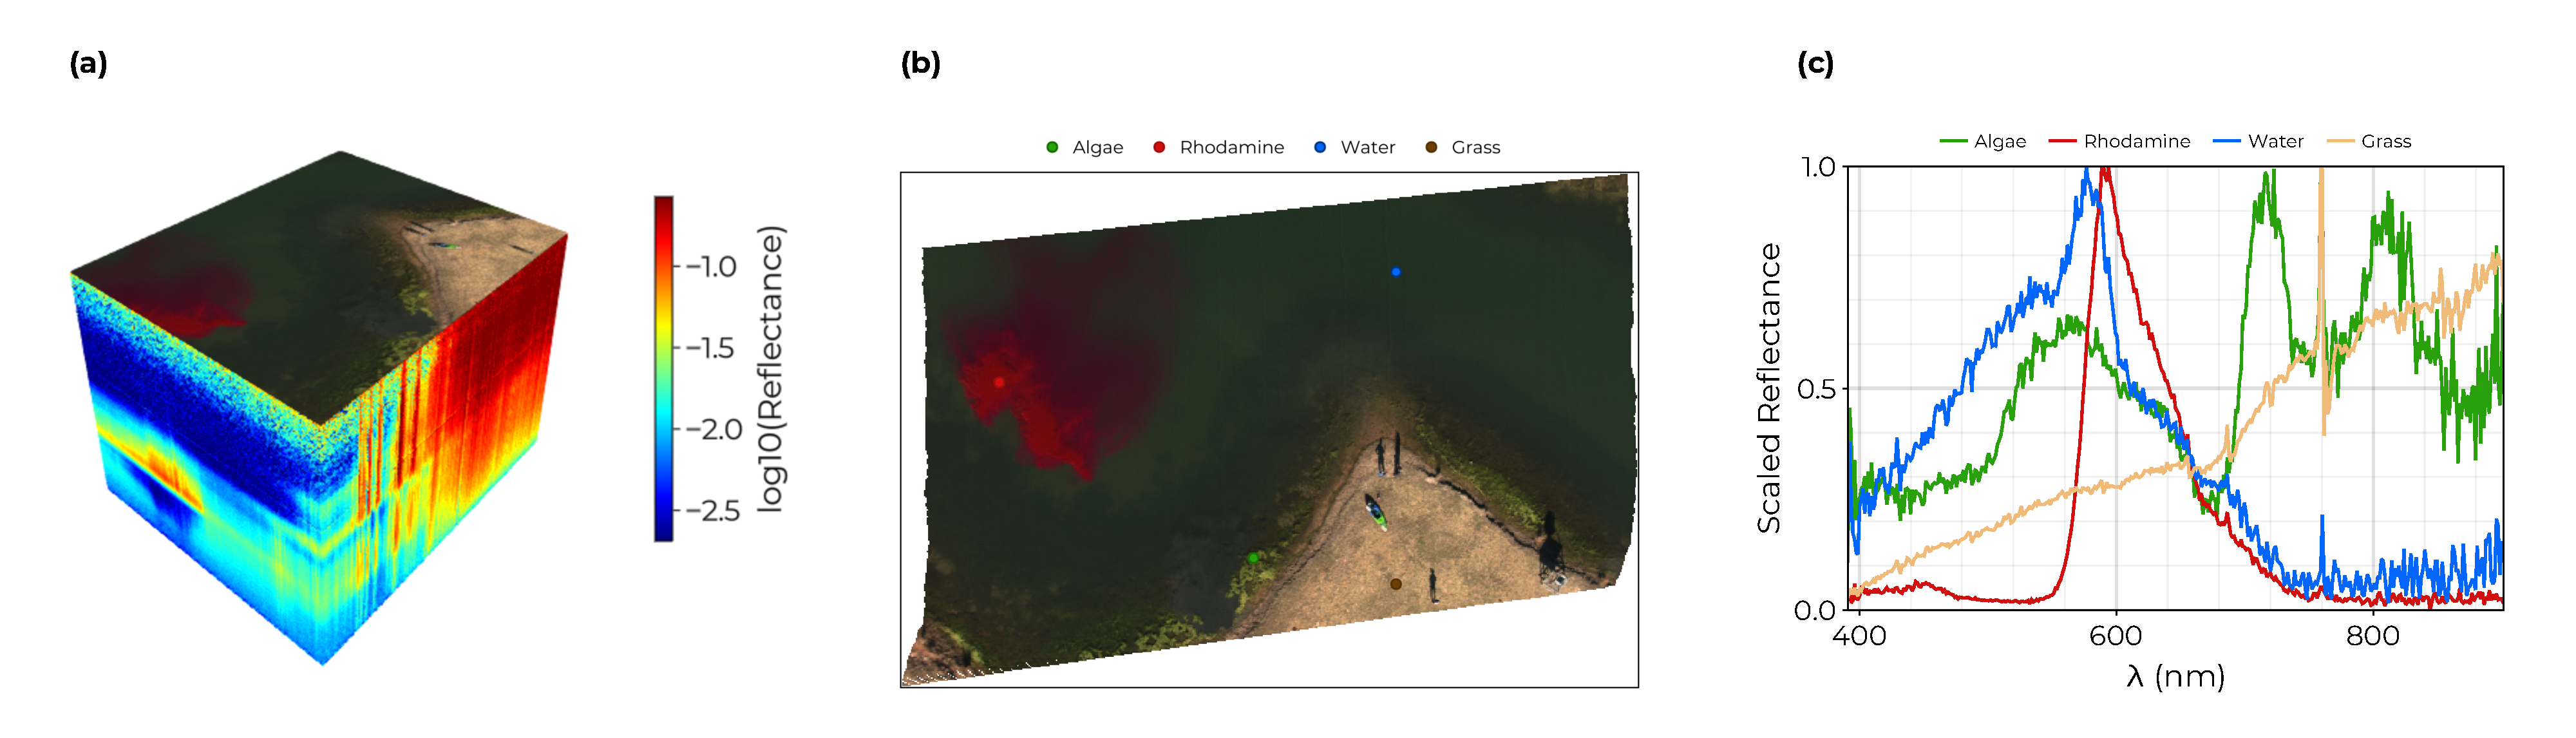
\includegraphics[width=15.5cm]{paper/figures/methods/sample-spectra.pdf}
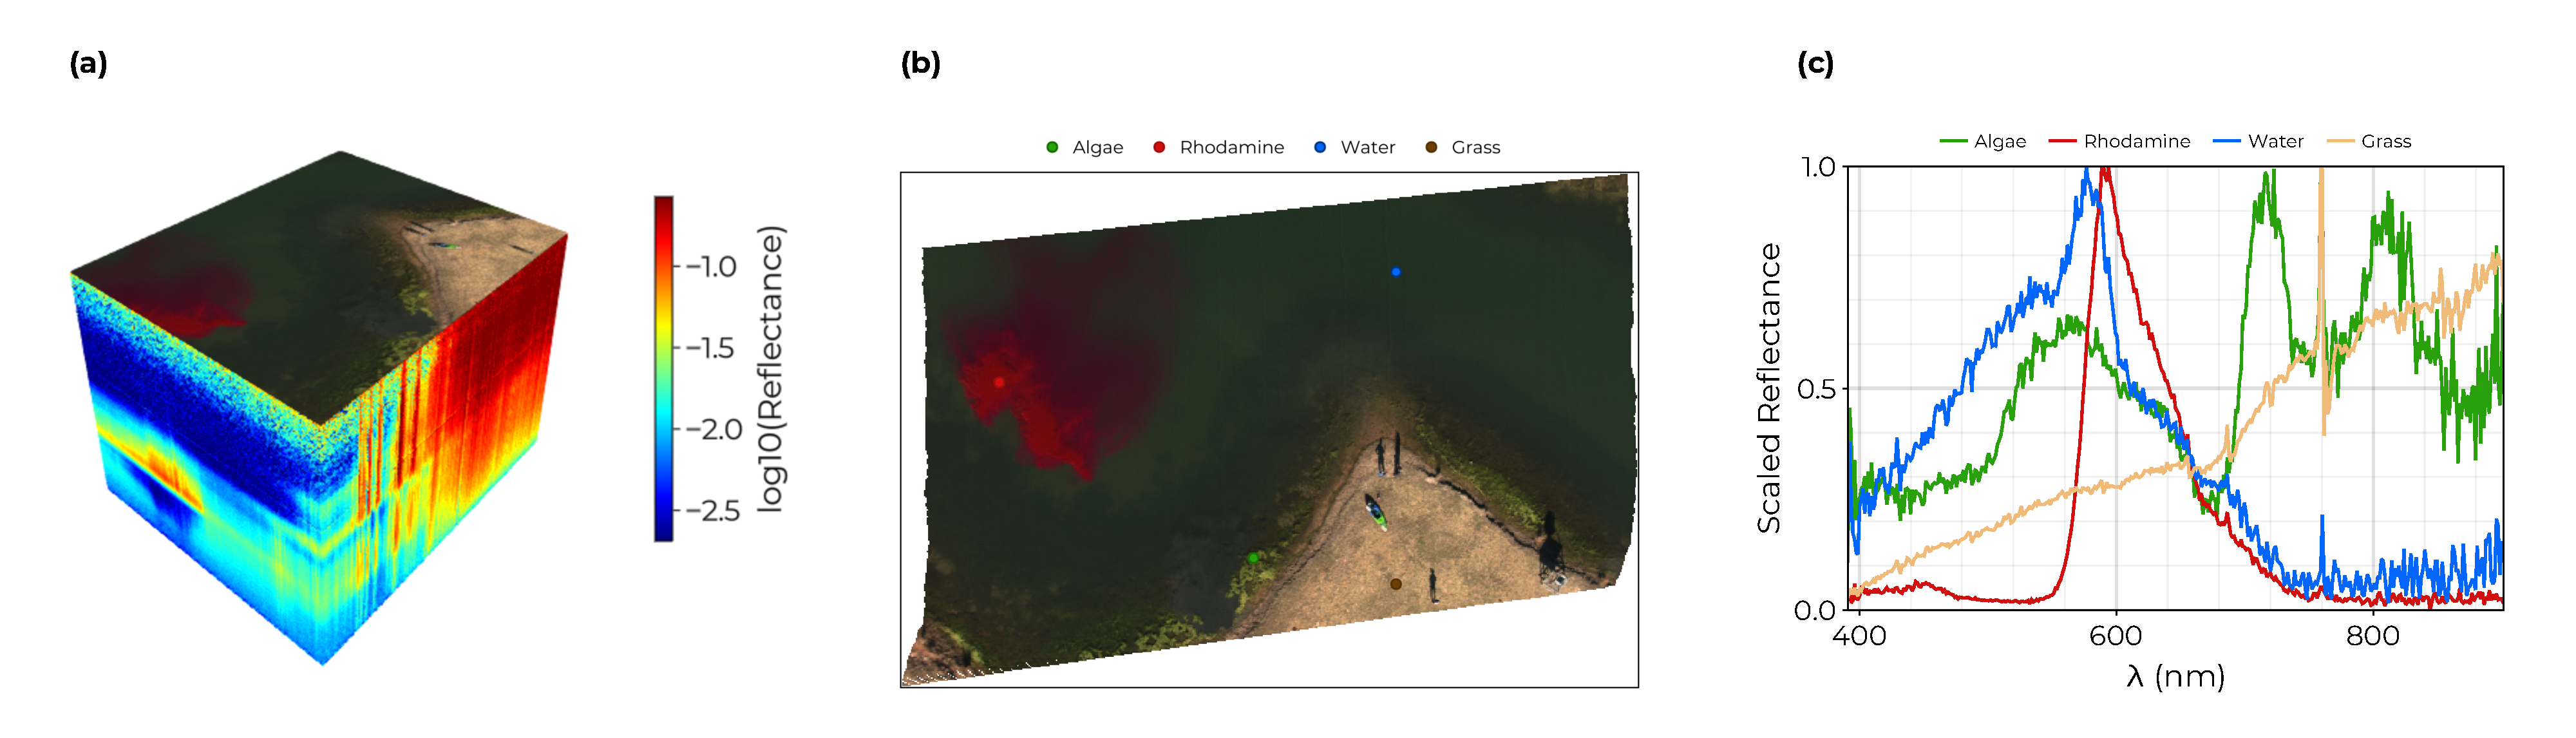
\includegraphics[width=\columnwidth]{paper/figures/methods/sample-spectra.pdf}
%\end{adjustwidth}
\caption{(a) Sample hyperspectral data cube. Spectra are plotted using their geographic position with the log10-reflectance colored along the z axis and a pseudo-color image on top. (b) Points taken from a sample hyperspectral data cube corresponding to algae, rhodamine dye, water, and dry grass. (c) The associated spectra for the exemplar points scaled so that the peak value of each spectrum is 1. (d) The location of the pond in Montague, Texas where data were collected for this study.\label{fig:sample-spectra}}
\end{figure}  


\subsection{Autonomous Robot Team}
\subsection{Data Collection and Pre-Processing}
\subsection{Generative Topographic Mapping}

- GTM paper oricinal \cite{gtm-bishop-1}
- GTM developments paper \cite{gtm-biship-2}


\subsection{Image Segmentation with the Normalized Spectral Similarity Score}

%%%%%%%%%%%%%%%%%%%%%%%%%%%%%%%%%%%%%%%%%%
\section{Results}

\subsection{GTM Fit}

\begin{figure}[t]
\centering
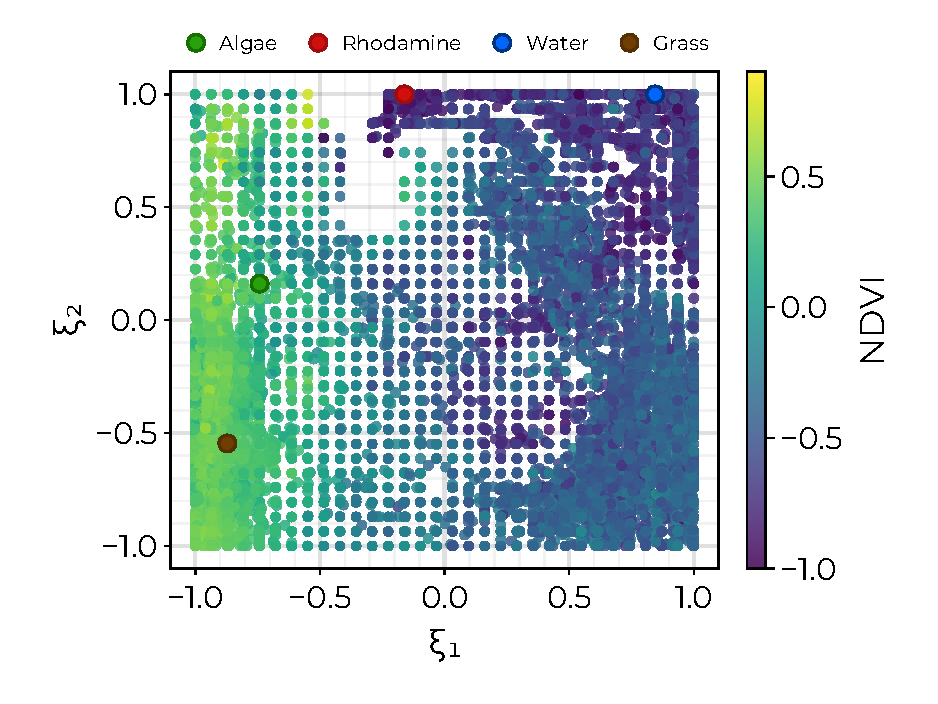
\includegraphics[width=0.8\columnwidth]{paper/figures/results/square-ndvi.pdf}
\caption{GTM Map: We plot the mean position of each data point in the latent space with points colored by the their associated NDVI values. The locations of the exemplar points for algae, rhodamine dye, water, and dry grass are shown in the latent space illustrating that the GTM has clearly distinguished land, near-land, and water pixels.\label{fig:}}
\end{figure}  


\subsection{Hyperparamter Optimization with BIC}


\begin{figure}[t]
%\begin{adjustwidth}{-\extralength}{0cm}
\centering
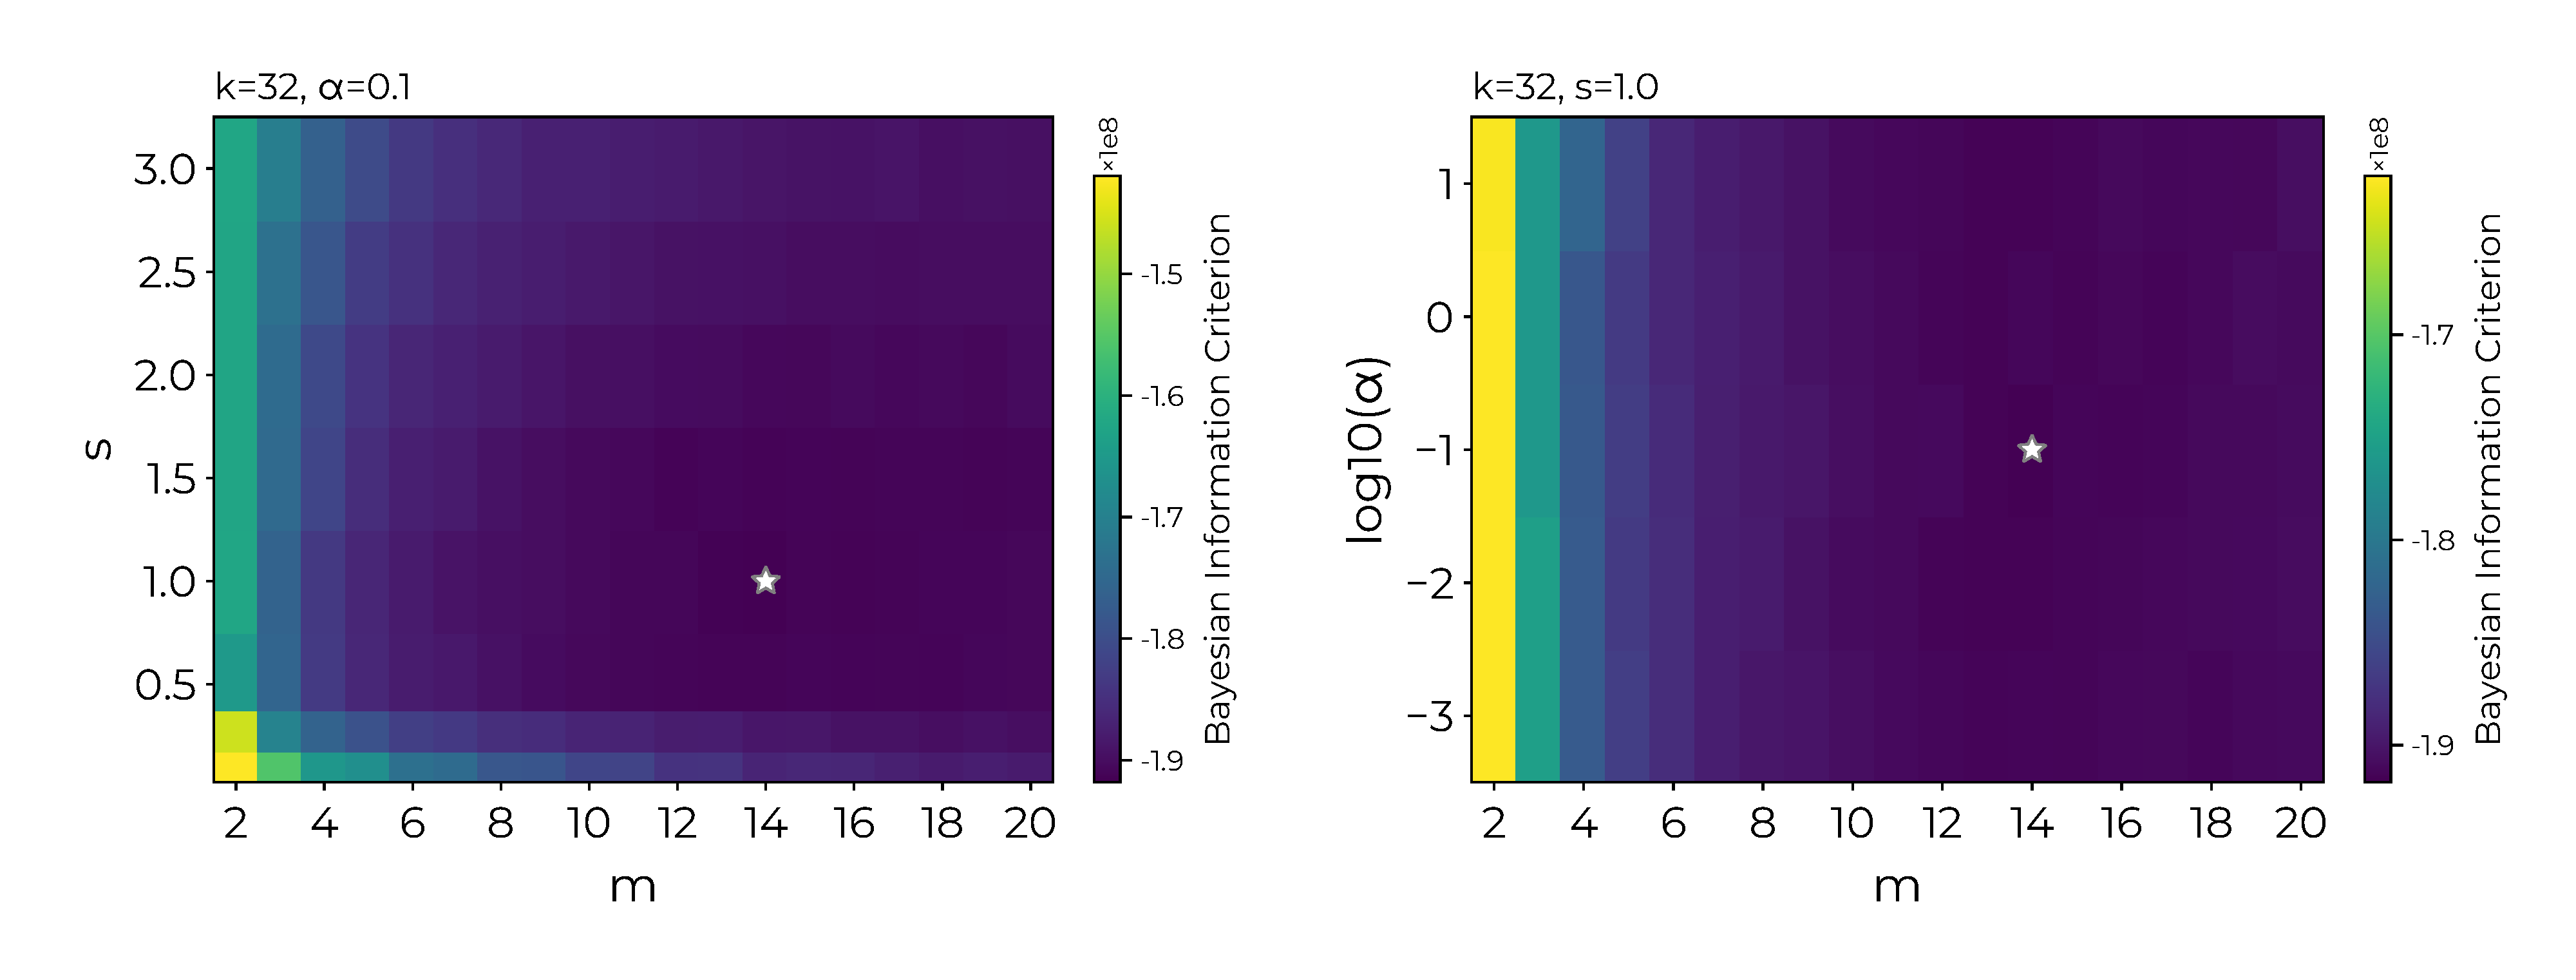
\includegraphics[width=\textwidth]{paper/figures/results/bic.pdf}
%\end{adjustwidth}
\caption{Results of the hyperparameter search. Left: Variation of BIC with $m$ and $s$ for fixed $\alpha=0.1$. Right: Variation of the BIC with with $m$ and $\alpha$ for fixed $s=1.0$. The white star in each plot indicates the parameters with the lowest BIC.\label{fig:hp-results}}
\end{figure}  


\subsection{Spectral Signatures}


\begin{figure}[t]
\begin{adjustwidth}{-\extralength}{0cm}
\centering
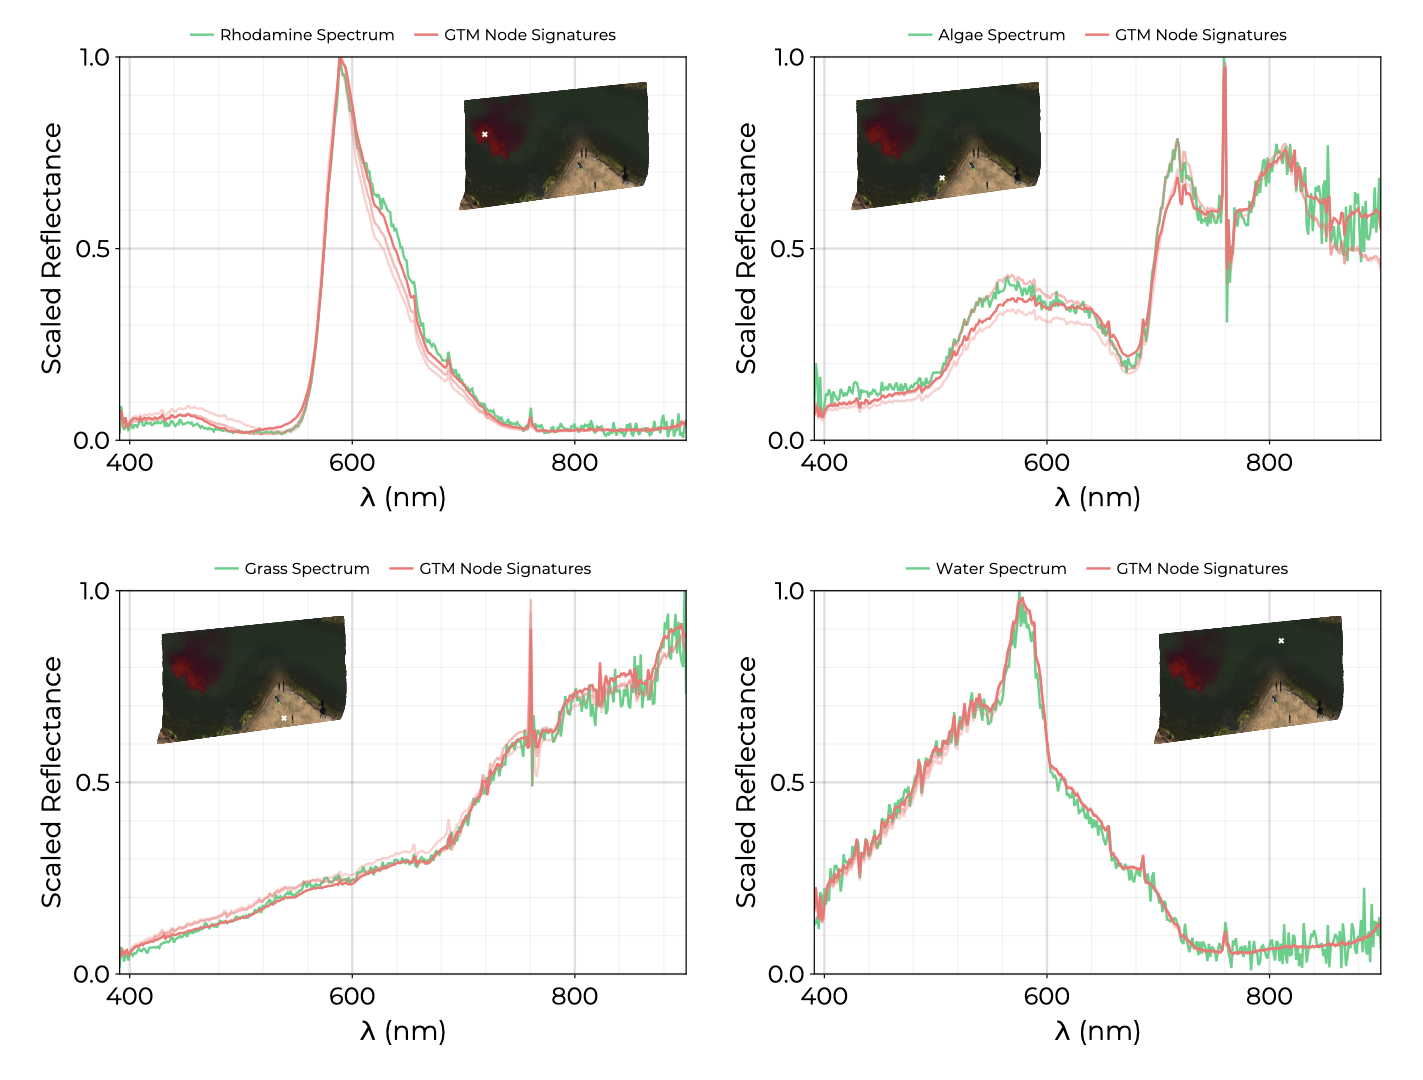
\includegraphics[width=15.5cm]{paper/figures/results/spectral-signatures.png}
\end{adjustwidth}
\caption{GTM Node Signatures corresponding to the exemplar spectra for the rhodamine plume (top left), algae (top right), dry grass (bottom left), and open water (bottom right). \label{fig:spectral-signautes}}
\end{figure}  

\subsection{Water Class Map}

\begin{figure}[t]
\begin{adjustwidth}{-\extralength}{0cm}
\centering
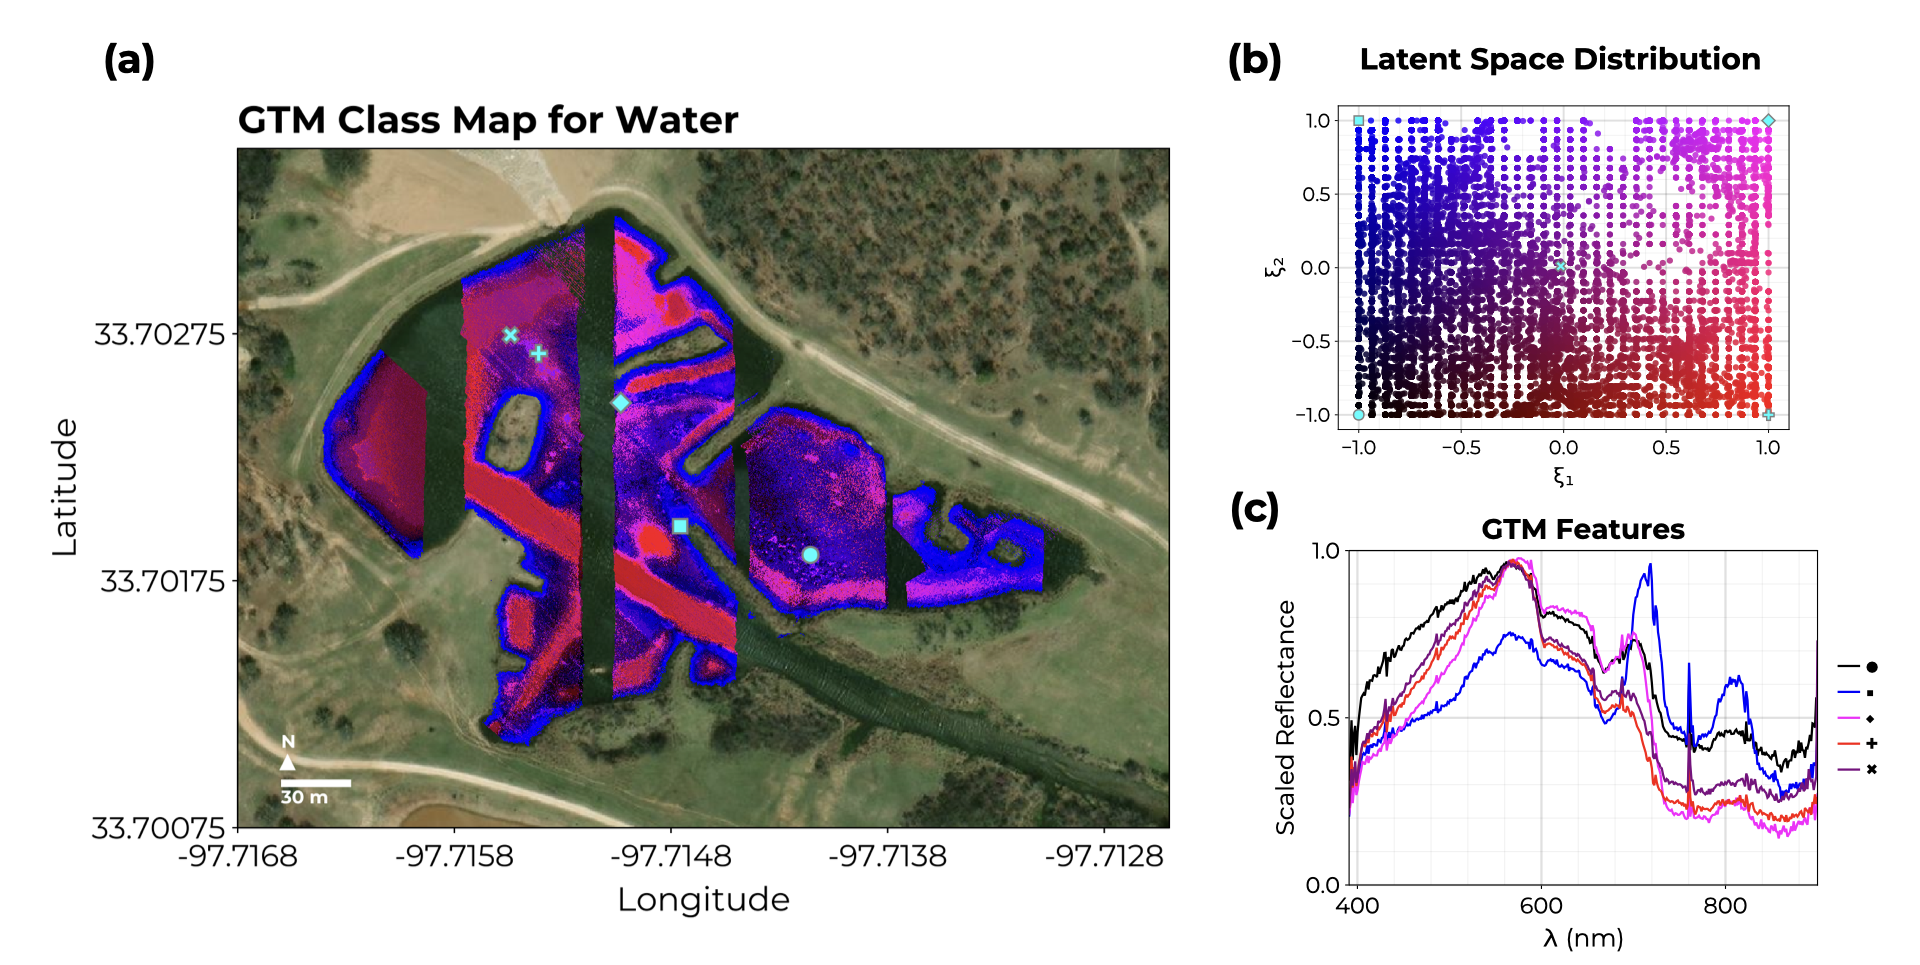
\includegraphics[width=18.0cm]{paper/figures/results/gtm-water.png}
\end{adjustwidth}
\caption{Classification map for GTM trained solely on water pixels (no land and no rhodamine plume). \textbf{(a)} GTM applied to all water pixels colored by their associated position in the latent space. \textbf{(b)} Representation of the poitns from the training set in the latent space. The points are colored with $\xi_1$ corresponding to red and $\xi_2$ corresponding to blue. \textbf{(c)} The associated GTM spectral signatures, $\Psi_i$, corresponding to the four corners and center of the GTM latent space. \label{fig:gtm-water}}
\end{figure}  


\subsection{Algae Identification}


\begin{figure}[t]
\begin{adjustwidth}{-\extralength}{0cm}
\centering
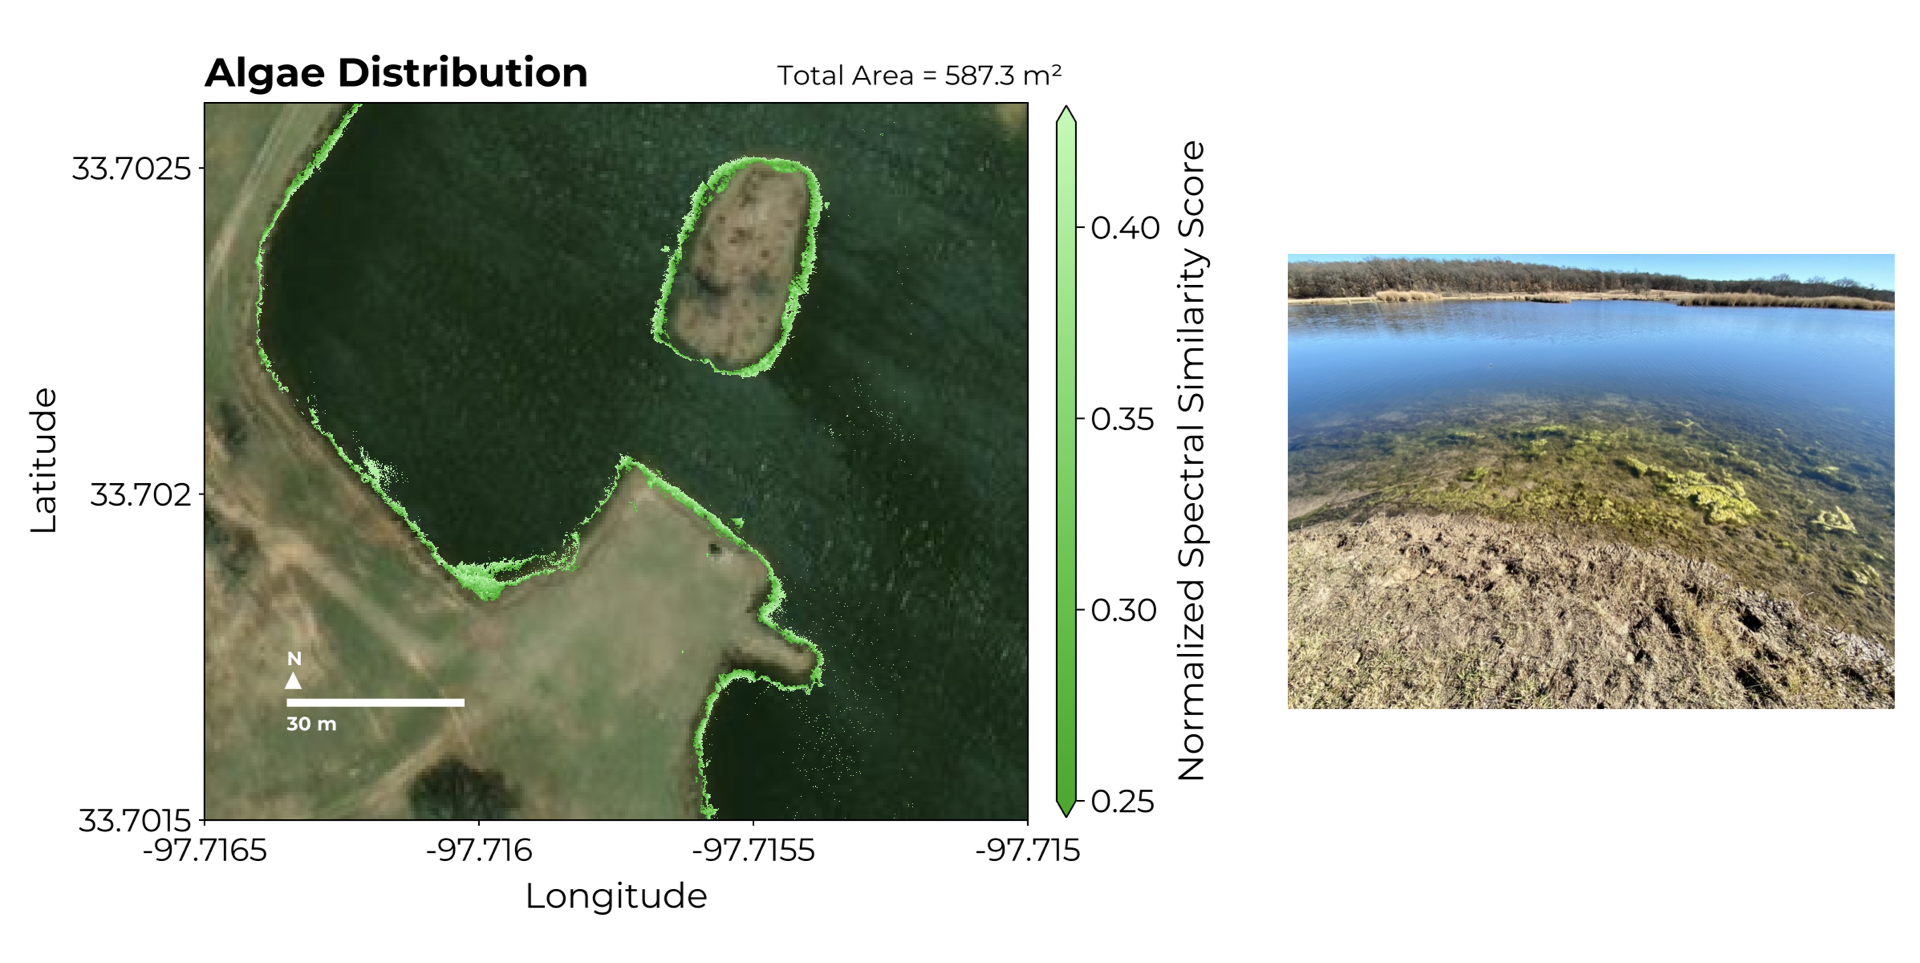
\includegraphics[width=15.5cm]{paper/figures/results/algae.png}
\end{adjustwidth}
\caption{\label{fig:algae-map}}
\end{figure}  



\subsection{Rhodamine Dye Plume Identification}

\begin{figure}[t]
\begin{adjustwidth}{-\extralength}{0cm}
\centering
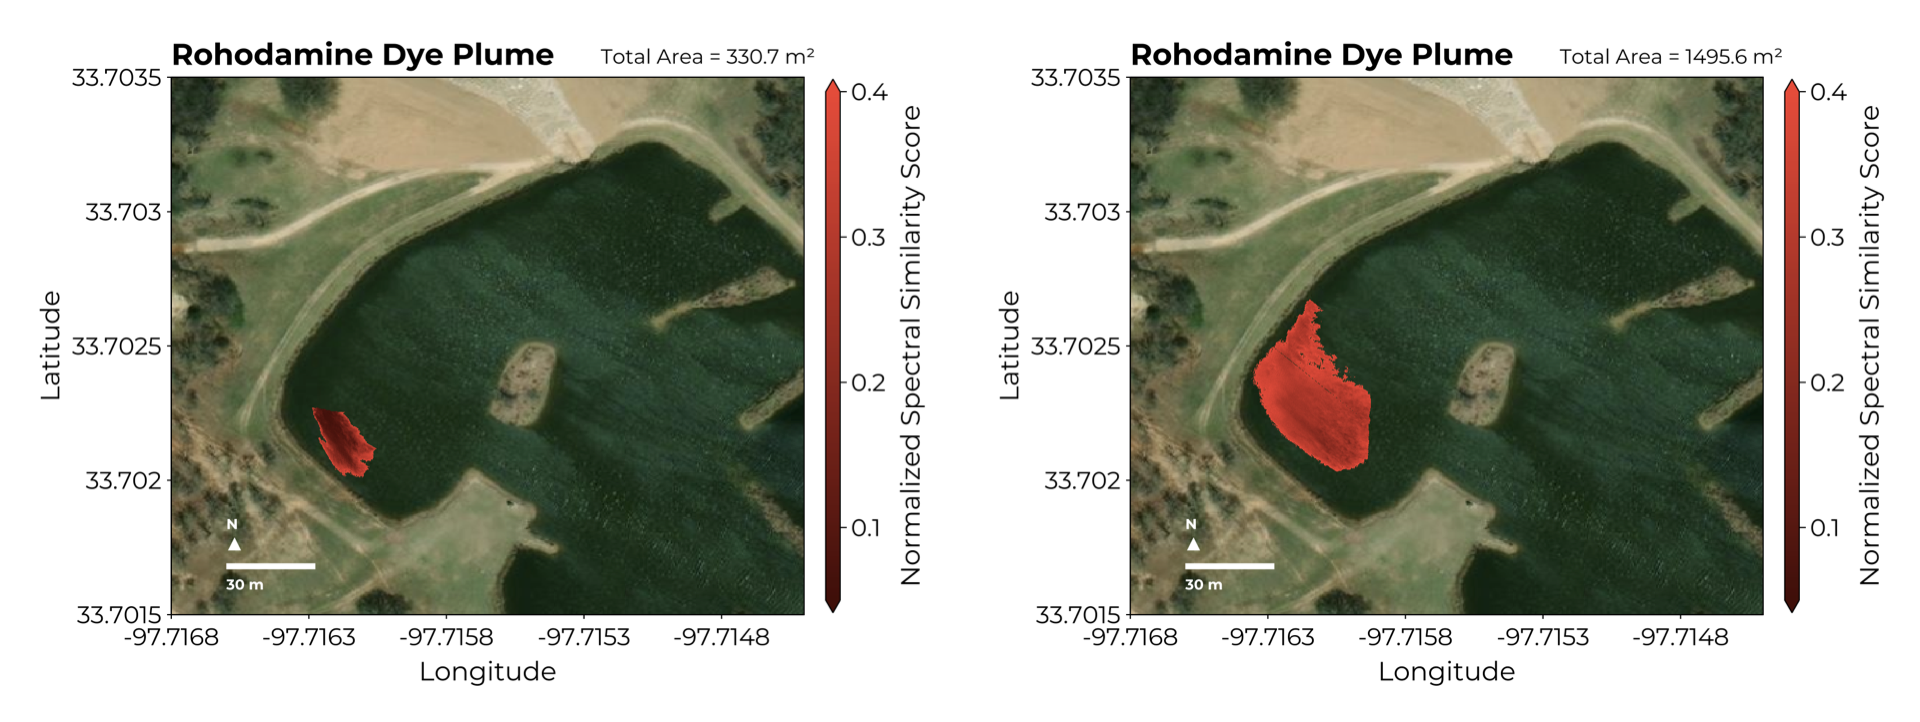
\includegraphics[width=15.5cm]{paper/figures/results/rhodamine.png}
\end{adjustwidth}
\caption{\label{fig:rhodamine-map}}
\end{figure}  




%%%%%%%%%%%%%%%%%%%%%%%%%%%%%%%%%%%%%%%%%%
\section{Discussion}

\subsection{Summary of GTM applications in our paper}
\subsection{Comparison to other existing approaches in literature}
- Is there much done for classification in real time? 
\subsection{Other applications of GTM}
- Discuss use of GTM means/modes/responsibilities feature transformer for supervised models (e.g. better than PCA) 
- Use of GTM classes to aid autonomous data collection by identification of "interesting" regons


%%%%%%%%%%%%%%%%%%%%%%%%%%%%%%%%%%%%%%%%%%
\section{Conclusions}


%%%%%%%%%%%%%%%%%%%%%%%%%%%%%%%%%%%%%%%%%%
\vspace{6pt} 

%%%%%%%%%%%%%%%%%%%%%%%%%%%%%%%%%%%%%%%%%%
%% optional
%\supplementary{The following supporting information can be downloaded at:  \linksupplementary{s1}, Figure S1: title; Table S1: title; Video S1: title.}

% Only for journal Methods and Protocols:
% If you wish to submit a video article, please do so with any other supplementary material.
% \supplementary{The following supporting information can be downloaded at: \linksupplementary{s1}, Figure S1: title; Table S1: title; Video S1: title. A supporting video article is available at doi: link.}

% Only for journal Hardware:
% If you wish to submit a video article, please do so with any other supplementary material.
% \supplementary{The following supporting information can be downloaded at: \linksupplementary{s1}, Figure S1: title; Table S1: title; Video S1: title.\vspace{6pt}\\
%\begin{tabularx}{\textwidth}{lll}
%\toprule
%\textbf{Name} & \textbf{Type} & \textbf{Description} \\
%\midrule
%S1 & Python script (.py) & Script of python source code used in XX \\
%S2 & Text (.txt) & Script of modelling code used to make Figure X \\
%S3 & Text (.txt) & Raw data from experiment X \\
%S4 & Video (.mp4) & Video demonstrating the hardware in use \\
%... & ... & ... \\
%\bottomrule
%\end{tabularx}
%}

%%%%%%%%%%%%%%%%%%%%%%%%%%%%%%%%%%%%%%%%%%
\authorcontributions{FIXME}

\funding{FIXME}

\institutionalreview{Not applicable}

\informedconsent{Not applicable}

\dataavailability{We encourage all authors of articles published in MDPI journals to share their research data. In this section, please provide details regarding where data supporting reported results can be found, including links to publicly archived datasets analyzed or generated during the study. Where no new data were created, or where data is unavailable due to privacy or ethical restrictions, a statement is still required. Suggested Data Availability Statements are available in section ``MDPI Research Data Policies'' at \url{https://www.mdpi.com/ethics}.} 


\acknowledgments{In this section you can acknowledge any support given which is not covered by the author contribution or funding sections. This may include administrative and technical support, or donations in kind (e.g., materials used for experiments).}

\conflictsofinterest{Declare conflicts of interest or state ``The authors declare no conflicts of interest.'' Authors must identify and declare any personal circumstances or interest that may be perceived as inappropriately influencing the representation or interpretation of reported research results. Any role of the funders in the design of the study; in the collection, analyses or interpretation of data; in the writing of the manuscript; or in the decision to publish the results must be declared in this section. If there is no role, please state ``The funders had no role in the design of the study; in the collection, analyses, or interpretation of data; in the writing of the manuscript; or in the decision to publish the results''.} 

%%%%%%%%%%%%%%%%%%%%%%%%%%%%%%%%%%%%%%%%%%
%% Optional

%% Only for journal Encyclopedia
%\entrylink{The Link to this entry published on the encyclopedia platform.}

\abbreviations{Abbreviations}{
The following abbreviations are used in this manuscript:\\

\noindent 
\begin{tabular}{@{}ll}
MDPI & Multidisciplinary Digital Publishing Institute\\
DOAJ & Directory of open access journals\\
TLA & Three letter acronym\\
LD & Linear dichroism
\end{tabular}
}

%%%%%%%%%%%%%%%%%%%%%%%%%%%%%%%%%%%%%%%%%%
%% Optional
\appendixtitles{yes} % Leave argument "no" if all appendix headings stay EMPTY (then no dot is printed after "Appendix A"). If the appendix sections contain a heading then change the argument to "yes".
\appendixstart
\appendix
\section[\appendixname~\thesection]{Hyperparameter Search Results}

\begin{table}[H]
  \caption{The top 25 models from the hyperparameter search. A variety of GTM were trained to explore the the impact of varying m, $\alpha$, and s.\label{tab:hp-search}}
  \begin{adjustwidth}{-\extralength}{0cm}
  \newcolumntype{C}{>{\centering\arraybackslash}X}
  \begin{tabularx}{\fulllength}{CCCCCC}
    \toprule
    \textbf{m} & \textbf{$\alpha$} & \textbf{s} & \textbf{k} & \textbf{BIC} & \textbf{AIC} \\
    \midrule
    14 & 0.1 & 1.0 & 32 & \textbf{-1.918e8} & -1.926e8\\
    13 & 0.01 & 1.0 & 32 & -1.917e8 & -1.923e8\\
    16 & 0.01 & 1.5 & 32 & -1.917e8 & -1.926e8\\
    14 & 10.0 & 1.0 & 32 & -1.917e8 & -1.924e8\\
    16 & 0.001 & 1.5 & 32 & -1.917e8 & -1.926e8\\
    13 & 1.0 & 1.0 & 32 & -1.917e8 & -1.923e8\\
    13 & 10.0 & 1.0 & 32 & -1.917e8 & -1.923e8\\
    14 & 0.001 & 1.5 & 32 & -1.916e8 & -1.924e8\\
    13 & 0.1 & 1.0 & 32 & -1.916e8 & -1.923e8\\
    14 & 0.01 & 1.0 & 32 & -1.916e8 & -1.924e8\\
    15 & 0.01 & 1.5 & 32 & -1.916e8 & -1.925e8\\
    14 & 0.01 & 1.5 & 32 & -1.916e8 & -1.923e8\\
    15 & 1.0 & 1.0 & 32 & -1.916e8 & -1.924e8\\
    18 & 0.01 & 1.5 & 32 & -1.916e8 & -1.928e8\\
    12 & 0.01 & 1.0 & 32 & -1.916e8 & -1.921e8\\
    15 & 0.01 & 0.5 & 32 & -1.915e8 & -1.924e8\\
    17 & 1.0 & 1.0 & 32 & -1.915e8 & -1.926e8\\
    16 & 0.1 & 1.0 & 32 & -1.915e8 & -1.925e8\\
    18 & 0.001 & 1.5 & 32 & -1.915e8 & -1.928e8\\
    13 & 0.001 & 1.0 & 32 & -1.915e8 & -1.922e8\\
    12 & 1.0 & 1.0 & 32 & -1.915e8 & -1.921e8\\
    17 & 0.001 & 1.5 & 32 & -1.915e8 & -1.926e8\\
    15 & 0.001 & 1.5 & 32 & -1.915e8 & -1.923e8\\
    15 & 10.0 & 1.0 & 32 & -1.915e8 & -1.923e8\\
    12 & 0.1 & 1.5 & 32 & -1.915e8 & -1.92e8\\
    \bottomrule
  \end{tabularx}
  \end{adjustwidth}
\end{table}


%%%%%%%%%%%%%%%%%%%%%%%%%%%%%%%%%%%%%%%%%%
\begin{adjustwidth}{-\extralength}{0cm}
%\printendnotes[custom] % Un-comment to print a list of endnotes

\reftitle{References}

%=====================================
% References, variant A: external bibliography
%=====================================
\bibliography{paper/references.bib}

%%%%%%%%%%%%%%%%%%%%%%%%%%%%%%%%%%%%%%%%%%
\PublishersNote{}
\end{adjustwidth}
\end{document}

